\chapter{Implementação Física}
\section{Seleção do sistema de gestão de bases de dados}
Optamos pela implementação duma base de dados usando o motor de base de dados MySQL.Trata-se dum motor de base de dados muito renomeado e quase padronizado pela industria, devido a sua elevada segurança dos dados, alto desempenho e pela sua capacidade de otimizar o programa reduzindo o tempo de execução. \par 
O MySQL ser um  motor de base de dados gratuito também contribuiu para a sua escolha, pois permite que seja possível a criação duma base de dados dentro dum orçamento mais amigável para o cliente.


\section{Tradução do esquema lógico para o sistema de gestão de bases de dados escolhido em SQL}

\begin{figure}[h]
\centering
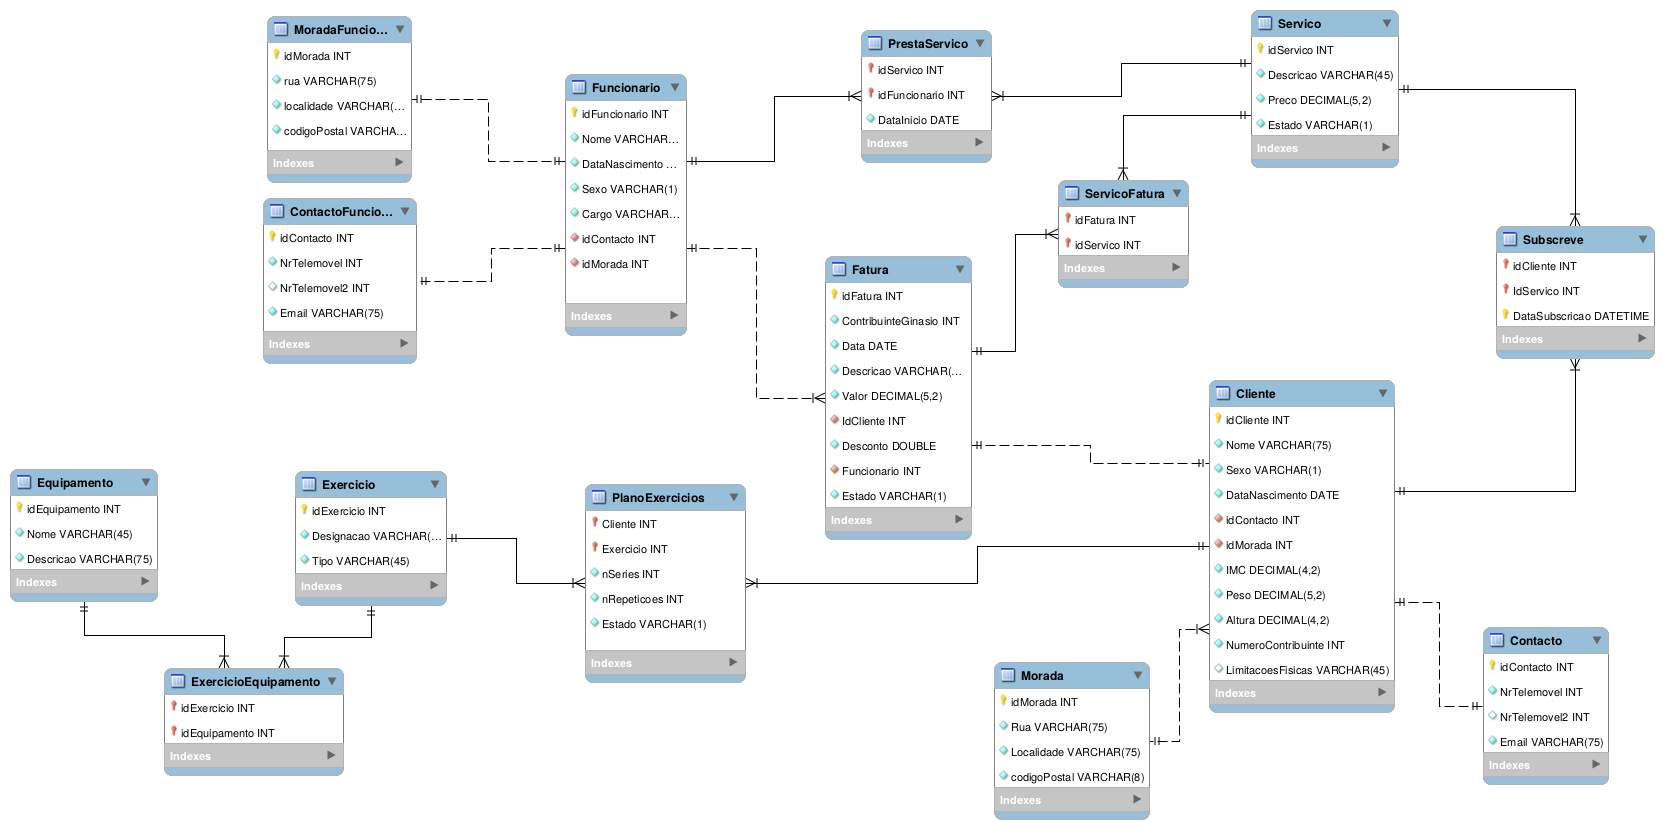
\includegraphics[width=\textwidth]{implementacao_fisica/ModeloLogico.png}
\caption{Modelo Lógico representado no MySQL Workbench}
\label{fig:mod_logico_mysql}
\end{figure}

\clearpage

\section{Tradução das interrogações do utilizador para SQL (alguns exemplos)}

\subsection{Interrogação faturação num mês}
\begin{lstlisting}[language=SQL]
    SELECT SUM(Valor) FROM Fatura as F
	    WHERE MONTH(F.Data)=01 AND YEAR(F.DATA)=2018; 
\end{lstlisting}

\begin{figure}[h]
\begin{center}
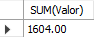
\includegraphics[scale=0.7]{implementacao_fisica/soma.png}
\centering
\end{center}
\end{figure}

\subsection{Todos os clientes que fizeram 'Martelo'}
\begin{lstlisting}[language=SQL]
SELECT IdCliente, Nome  FROM Cliente as C
	INNER JOIN planoexercicios as P on P.Cliente=C.idCliente
	INNER JOIN exercicio as E on P.Exercicio=E.idExercicio
	WHERE E.Designacao='Martelo';
\end{lstlisting}

\begin{figure}[h]
\begin{center}
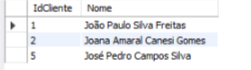
\includegraphics[scale=1.0]{implementacao_fisica/ClientesMartelo.png} 
\centering
\end{center}
\end{figure}

\subsection{A que serviços o cliente 1 está subscrito}
\begin{lstlisting}[language=SQL]
SELECT Descricao,nome  FROM Cliente as C
	INNER JOIN subscreve as S on C.idCliente=S.idCliente
    INNER JOIN servico as Z on S.Idservico=Z.idservico
    WHERE (C.idCliente=1);
\end{lstlisting}

\begin{figure}[h]
\begin{center}
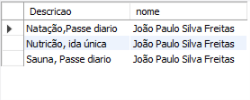
\includegraphics[scale=1.0]{implementacao_fisica/Servicoscliente1.png} 
\centering
\end{center}
\end{figure}

\subsection{Faturas correspondentes ao cliente 2}
\begin{lstlisting}[language=SQL]
SELECT idFatura,Valor FROM fatura as F
	INNER JOIN Cliente as C on F.idCliente=C.idCliente
    WHERE C.idCliente=2;
    
\end{lstlisting}
\begin{figure}[h]
\begin{center}
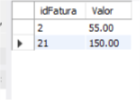
\includegraphics[scale=1.0]{implementacao_fisica/Desenho.png} 
\centering
\end{center}
\end{figure}

\section{Tradução das transações estabelecidas para SQL (alguns exemplos)}
Quando um cliente é criado, também é criado a morada e o seu contacto, usando as transações os contactos e a morada só são criados se e só se o cliente também for criado.
\begin{lstlisting}[language=SQL]

CREATE DEFINER=`root`@`localhost` PROCEDURE `Nova Ficha de Cliente`(in nome VARCHAR(75),in idade INT,in sexo VARCHAR(1),in peso INT, in altura INT,in numerocontribuinte INT, in limitacoesfisicas VARCHAR(75),in telemovel1 INT, in telemovel2 INT ,email VARCHAR(75),rua VARCHAR(75),localidade VARCHAR(75),codigopostal VARCHAR(75))
BEGIN
DECLARE x INT;
DECLARE y INT;
DECLARE z INT;
 DECLARE EXIT HANDLER FOR SQLEXCEPTION
   BEGIN
      ROLLBACK;
      RESIGNAL;
   END;

START TRANSACTION;


 SET z = peso /POWER(altura,2);
INSERT INTO morada
	(Rua,Localidade,codigoPostal)
    VALUES
		(rua,localidade,codigopostal);
 SET x=  LAST_INSERT_ID();
        
INSERT INTO contacto
		(NrTelemovel,NrTelemovel2,Email)
        Values
			(telemovel1,telemovel2,email);
SET y=LAST_INSERT_ID();
INSERT INTO cliente
	(Nome,Sexo,Idade,idContacto,IdMorada,IMC,Peso,Altura,NumeroContribuinte,LimitacoesFisicas)
    Values
		(nome,sexo,idade,x,y,z,peso,altura,numerocontribuinte,limitacoesfisicas);
        COMMIT;
 END
\end{lstlisting}
\clearpage
Tal como nos clientes, nos apenas podemos adicionar o contacto e a morada do funcionario se a adição do funcionario também foi um sucesso
\begin{lstlisting}[language=SQL]
CREATE DEFINER=`root`@`localhost` PROCEDURE `Criacao da Ficha de novo Funcionario`(in nome VARCHAR(75),in idade INT,in sexo VARCHAR(1),in cargo VARCHAR(75),in telemovel1 INT, in telemovel2 INT ,email VARCHAR(75),rua VARCHAR(75),localidade VARCHAR(75),codigopostal VARCHAR(75))
BEGIN
DECLARE x INT;
DECLARE y INT;
DECLARE EXIT HANDLER FOR SQLEXCEPTION
   BEGIN
      ROLLBACK;
      RESIGNAL;
   END;
   START TRANSACTION;
INSERT INTO moradafuncionario
	(Rua,Localidade,codigoPostal)
    VALUES
		(rua,localidade,codigopostal);

SET x=  LAST_INSERT_ID();
        
INSERT INTO contactofuncionario
		(NrTelemovel,NrTelemovel2,Email)
        Values
			(telemovel1,telemovel2,email);
SET y=LAST_INSERT_ID();
INSERT INTO funcionario
	(Nome,Idade,Sexo,Cargo,idContacto,IdMorada)
    Values
		(nome,idade,sexo,cargo,y,x);
COMMIT;
END
\end{lstlisting}

\section{Escolha, definição e caracterização de índices em SQL (alguns exemplos)}
Implementamos um índice no nosso Plano de Exercícios uma vez que é uma tabela que ao longo do tempo vai ficar extremamente populada, pois para cada cliente vamos preencher vários exercícios, como tal para encontrar o plano de exercícios dum cliente criamos um índice na coluna do idCliente para facilitar a sua procura.
\par Pensamos ainda implementar um índice na tabela dos clientes, mas como ainda se trata dum pequeno ginásio, a expectativa de número de clientes não justifica a implementação dum índice. 

\clearpage
\section{Estimativa do espaço em disco da base de dados e taxa de crescimento anual}
Para a estrutura de base de dados no seu estado atual e considerando os tamanhos máximos permitidos nas várias estruturas, temos uma ocupação máxima  de espaço dividida para cada elemento inserido.

\vspace{15pt}
\noindent
\textbf{Exemplo de cálculo do espaço ocupado:}

\begin{table}[h]
\resizebox{\textwidth}{!}{
\begin{tabular}{|l|c|}
\hline
\multicolumn{1}{|c|}{\textbf{Espaço ocupado pela tabela Cliente}}                                                                                                                                                                                               & \multicolumn{1}{l|}{\textbf{Total em Bytes}} \\ \hline
Primeiro de tudo, o Cabeçalho, ocupa 4 bytes.                                                                                                                                                                                        & 4 bytes                                      \\ \hline
Data Type que tem valor fixo(INT)5x4                                                                                                                                                                                                 & 20 bytes                                     \\ \hline
Null Block = 2 bytes, pois temos 11 campos                                                                                                                                                                                           & 2 bytes                                      \\ \hline
Variable Block = 2 bytes + 12bytes (2 para cada campo com dados variáveis, nos temos 6)                                                                                                                                              & 14 bytes                                     \\ \hline
\begin{tabular}[c]{@{}l@{}}Data Types com valores variáveis (nome varchar(75),sexo varchar(1),IMC decimal(4,2), \\                              Peso decimal(5,2), altura(decimal(4,2) e limitações físicas varchar(45)\end{tabular} & 134 bytes                                    \\ \hline
\textbf{Total}                                                                                                                                                                                                                       & 174 bytes                                    \\ \hline
\end{tabular}
}
\end{table}
\begin{itemize}
\item Um cliente ocupa 174bytes+96bytes do contacto +  175bytes da morada,ou seja, 445 bytes
\item Um funcionário ocupa 154 bytes +96bytes para contacto + 175 bytes para a morada,ou seja,425 bytes
\item Uma fatura ocupa 149 bytes
\item Um serviço ocupa 68 bytes
\item Um exercício ocupa 135 bytes
\item Um equipamento ocupa 138 bytes
\item Uma relação entre serviço e funcionário ocupa 15 bytes
\item Uma relação entre serviço e cliente ocupa  23 bytes
\item Uma relação entre serviço e fatura ocupa 15 bytes
\item Uma relação entre cliente e exercício ocupa 23 bytes
\item Uma relação entre exercício e equipamento ocupo 15 bytes

Tendo em conta que a base de dados no estado atual tem 20 clientes, 8 funcionários,9 serviços, 18 equipamentos, 22 exercícios, 82 exercícios dedicados aos clientes ,6 serviços a ser prestados aos clientes pelos funcionários, existem 35 inscrições dos clientes nos serviços,20 serviços faturados,23 exercícios utilizam equipamento e 20 faturas, temos :

\begin{lstlisting}[literate=%
        {é}{{\'{e}}}1
        {è}{{\`{e}}}1
        {ê}{{\^{e}}}1
        {ë}{{\¨{e}}}1
        {É}{{\'{E}}}1
        {Ê}{{\^{E}}}1
        {û}{{\^{u}}}1
        {ù}{{\`{u}}}1
        {ú}{{\'{u}}}1
        {â}{{\^{a}}}1
        {à}{{\`{a}}}1
        {á}{{\'{a}}}1
        {ã}{{\~{a}}}1
        {Á}{{\'{A}}}1
        {Â}{{\^{A}}}1
        {Ã}{{\~{A}}}1
        {ç}{{\c{c}}}1
        {Ç}{{\c{C}}}1
        {õ}{{\~{o}}}1
        {ó}{{\'{o}}}1
        {ô}{{\^{o}}}1
        {Õ}{{\~{O}}}1
        {Ó}{{\'{O}}}1
        {Ô}{{\^{O}}}1
        {î}{{\^{i}}}1
        {Î}{{\^{I}}}1
        {í}{{\'{i}}}1
        {Í}{{\~{Í}}}1]

20 x 445= 8900 B -> Clientes

8 x 425 = 3400 B -> Funcionário
9 x 68 = 612 B -> Serviço
18 x 138 = 2484 B -> Equipamento 
22 x 135 = 2970 B -> Exercícios
82 x 23 =1886 B -> Relacionamento exercício-cliente
6 x 15 =90 B -> Relacionamento serviço-funcionário
35 x 23 =805 B -> Relacionamento serviço-cliente
20 x 15 =300 B -> Relacionamento serviço-fatura
23 x 15 =345 B -> Relacionamento exercício-equipamento
20 x 149 = 2980 B -> Faturas

Total: 24 772 b = 24.19141 kB
\end{lstlisting}


Logo, a base de dados no estado atual tem aproximadamente 24.2kB ocupados.
\clearpage
O Sr. Miguel espera no próximo ano ter mais uma centena de clientes,subscrevendo se no mínimo a 1 serviço, cada um com pelo menos 5 exercícios( no intuito de balancear com os que se inscrevem apenas em nutrição,logo não tem exercícios), e para satisfazer as necessidades dos mesmos ele quer acrescentar 20 novos equipamentos e recrutar 5 novos funcionários, alem disso, planeia ter 2000 faturas ao final do ano.

\begin{lstlisting}[literate=%
        {é}{{\'{e}}}1
        {è}{{\`{e}}}1
        {ê}{{\^{e}}}1
        {ë}{{\¨{e}}}1
        {É}{{\'{E}}}1
        {Ê}{{\^{E}}}1
        {û}{{\^{u}}}1
        {ù}{{\`{u}}}1
        {ú}{{\'{u}}}1
        {â}{{\^{a}}}1
        {à}{{\`{a}}}1
        {á}{{\'{a}}}1
        {ã}{{\~{a}}}1
        {Á}{{\'{A}}}1
        {Â}{{\^{A}}}1
        {Ã}{{\~{A}}}1
        {ç}{{\c{c}}}1
        {Ç}{{\c{C}}}1
        {õ}{{\~{o}}}1
        {ó}{{\'{o}}}1
        {ô}{{\^{o}}}1
        {Õ}{{\~{O}}}1
        {Ó}{{\'{O}}}1
        {Ô}{{\^{O}}}1
        {î}{{\^{i}}}1
        {Î}{{\^{I}}}1
        {í}{{\'{i}}}1
        {Í}{{\~{Í}}}1]
        
100 x 445 = 44500 B-> Clientes
5 x 425 = 2125 B-> Funcionários
20 x 138 = 2760 B-> Equipamento
2000 x 149 = 298000 B-> Fatura
100 x 805 =  80500 B-> Relacionamento serviço-cliente
5 x 100 x 23 = 11500 B -> Relacionamento cliente-exercício
Total = 450885 B = 440.32 kB
\end{lstlisting}
\par Com base nestes dados no próximo ano a base de dados ocupará  24.1 + 440.32 =463.33 kB



\end{itemize}

\section{Definição e caracterização das vistas de utilização em SQL (alguns exemplos)}
Código da implementação da view que lista todos os clientes do Ginásio
\begin{lstlisting}[language=SQL]
CREATE VIEW `view_cliente` AS
    SELECT 
        C.idCliente,
        C.Nome,
        C.Sexo,
        C.Idade,
        C.IMC,
        C.Peso,
        C.Altura,
        C.NumeroContribuinte,
        C.LimitacoesFisicas,
        CC.NrTelemovel,
        CC.NrTelemovel2,
        CC.Email,
        M.Rua,
        M.Localidade,
        M.CodigoPostal
    FROM
        Cliente AS C
            INNER JOIN
        Contacto AS CC ON CC.idContacto = C.idContacto
            INNER JOIN
        Morada AS M ON M.idMorada = C.idMorada;
\end{lstlisting}

\begin{figure}[h]
\begin{center}
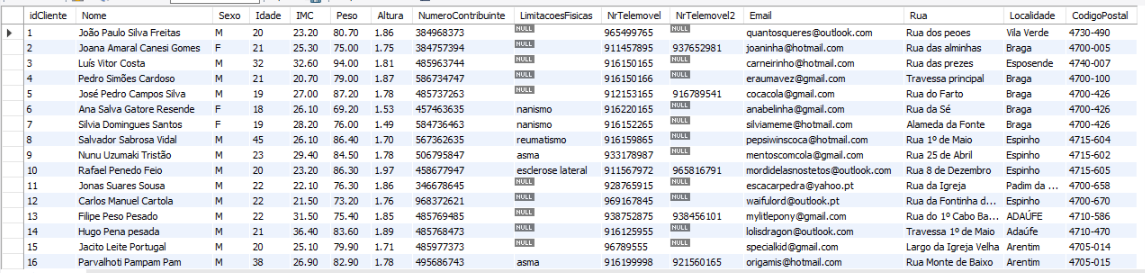
\includegraphics[scale=0.5]{implementacao_fisica/ViewCliente.png}
\centering
\end{center}
\end{figure}

\clearpage
Código da implementação da view que mostra todos os planos de exercícios.
\begin{lstlisting}[language=SQL]
CREATE VIEW `view_exerciciosCliente` AS

SELECT C.Nome AS NomeCliente, E.Designacao AS NomeExercicio, PE.nSeries,PE.nRepeticoes FROM PlanoExercicios AS PE
   INNER JOIN Exercicio AS E ON E.idExercicio = PE.Exercicio
   INNER JOIN Cliente AS C ON C.idCLiente = PE.Cliente;
\end{lstlisting}

\begin{figure}[h]
\begin{center}
%\includegraphics[scale=1.0]{implementacao_fisica/
\centering
\end{center}
\end{figure}
Código da implementação da view que mostra Os serviço(serviços que o cliente subscreveu) que cada funcionário faz
\begin{lstlisting}[language=SQL]
CREATE 
    ALGORITHM = UNDEFINED 
    DEFINER = `root`@`localhost` 
    SQL SECURITY DEFINER
VIEW `view_prestaservico` AS
    SELECT 
        `S`.`Descricao` AS `Descricao`,
        `F`.`Nome` AS `Nome`,
        `F`.`Cargo` AS `Cargo`,
        `S`.`Preco` AS `Preco`
    FROM
        ((`prestaservico` `PS`
        JOIN `servico` `S` ON ((`S`.`idServico` = `PS`.`idServico`)))
        JOIN `funcionario` `F` ON ((`F`.`idFuncionario` = `PS`.`idFuncionario`)))
    ORDER BY `S`.`Descricao`
\end{lstlisting}

\begin{figure}[h]
\begin{center}
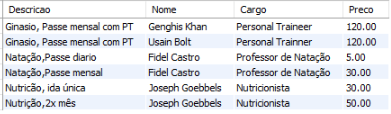
\includegraphics[scale=1.0]{implementacao_fisica/Prestaservico.png}
\centering
\end{center}
\end{figure}
\clearpage
Código da implementação da view que mostra a que serviços os clientes estão subscritos.
\begin{lstlisting}[language=SQL]
CREATE VIEW `view_subscricao` AS

SELECT C.Nome AS  NomeCliente, S.Descricao AS Servico, SUB.DataSubscricao FROM Subscreve AS SUB
   INNER JOIN Servico AS S ON S.idServico = SUB.idServico
   INNER JOIN Cliente AS C ON C.idCliente = SUB.idCliente;
\end{lstlisting}
\begin{figure}[h]
\begin{center}
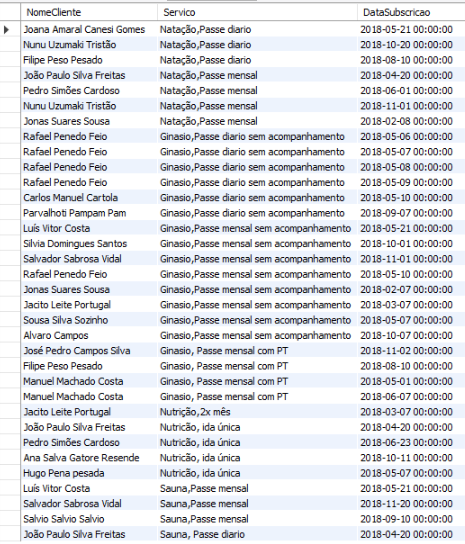
\includegraphics[scale=1.0]{implementacao_fisica/Susbricao.png}
\centering
\end{center}
\end{figure}
\clearpage
\section{Definição e caracterização dos mecanismos de segurança em SQL (alguns exemplos)}
Foram criados 2 users, um para cada rececionista , com apenas permissões de adicionar e dar update as linhas das tabelas, tenho como segurança que nenhum destes destroi uma tabela sem querer.
\begin{lstlisting}[language=SQL]
CREATE USER 'Jafar Strogonof'@'localhost' IDENTIFIED BY 'Jafar';

CREATE USER 'King Julian Move-it Move-it'@'localhost' IDENTIFIED BY 'Julian';

GRANT INSERT,UPDATE,EXECUTE, SHOW VIEW ON Ginasio.* TO 'Jafar Strogonof'@'localhost';
GRANT INSERT,UPDATE,EXECUTE, SHOW VIEW ON Ginasio.* TO 'King Julian Move-it Move-it'@'localhost';
\end{lstlisting}

\begin{figure}[h]
\begin{center}
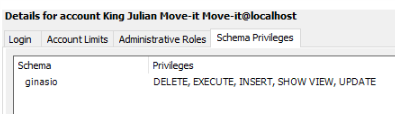
\includegraphics[scale=1.0]{implementacao_fisica/Previlegios.png}
\centering
\end{center}
\end{figure}
\par Sendo assim, o Sr. Miguel é a única pessoa com acesso administrativo a base de dados.

\section{Revisão do sistema implementado com o utilizador}
Após a implementação do sistema de base de dados, foi realizada uma reunião com o Sr.Miguel para ver se o produto final lhe agradava e receber algum feedback caso não estivesse do seu agrado.
\par Primeiramente o Sr.Miguel disse que não estávamos a cumprir completamente o seu pedido, ou seja, não tínhamos todos os procedimentos que este desejava, como por exemplo, adicionar um funcionário e um equipamento. Alargou-nos o prazo de entrega para a semana seguinte com o objetivo de  adicionarmos essas funções e para dar mais uns retoques onde fosse necessário.
\par Posteriormente, após a instalação e demonstração da execução destes novos procedimentos, o  Sr.Miguel ficou bastante satisfeito com o sistema de Base de Dados.